\documentclass[12pt] {article}
\usepackage{times}
\usepackage[margin=1in,bottom=1in,top=1in]{geometry}

\usepackage{hhline}
\usepackage{subfig}
\usepackage{amsmath}
\usepackage{amsfonts}
\usepackage[inline,shortlabels]{enumitem}%enumerate with letters
\usepackage{mathrsfs} 
\usepackage[square,numbers]{natbib}
\usepackage{graphicx}
\bibliographystyle{unsrtnat}

\usepackage[framed,numbered,autolinebreaks,useliterate]{./mcode}

\begin{document}

\title{Assignment Six -  EEC254}
\author{Ahmed H. Mahmoud}
\date{March 6th, 2018}
\maketitle

%============Table========
%\begin{figure}[tbh]
% \centering    
%\begin{tabular}{ |p{4cm}|| p{2cm}|p{2cm}|p{2cm}|p{2cm}|}
% \hline
% & Processor 1 &  Processor 2  & Processor 3 & Processor 4\\ \hhline{|=|=|=|=|=|}
% \hline
% Performance          &$1.08$        &$1.425$       &\textbf{1.52}  &   \\
% \hline
%\end{tabular} 
%\caption{Metric table for the four processors}
%   \label{tab:metric}
%\end{figure} 
%============Figure========
%\begin{figure}[!tbh]
%\centering        
%   \subfloat {\includegraphics[width=0.65\textwidth]{fig2_4.png}}
%   \caption{ }
%   \label{fig:fig}
%\end{figure}

%\begin{enumerate}[(a)]
%\end{enumerate}


\paragraph{Problem 9.30:} 
For this problem, we started with Newton method first. In order to validate the results, we plotted the contours of the objective function for $x\in \mathbb{R}^2$ i.e., $n=2$. Figure~\ref{fig:contours} shows the contours of the objective function for different $m$ along with the trajectory of $x$. It is clear that the implementation is correct and the trajectory of $x$ always minimizes the objective function. 

\begin{figure}[!tbh]
\centering        
   \subfloat {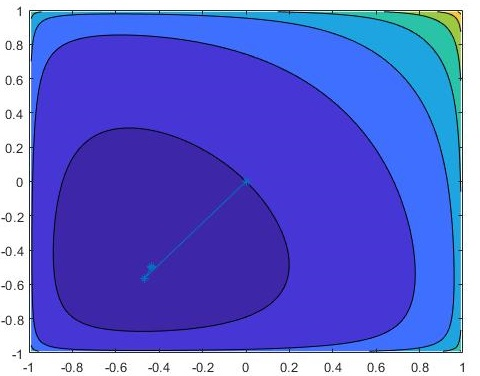
\includegraphics[width=0.24\textwidth]{code/5.jpg}}
   \subfloat {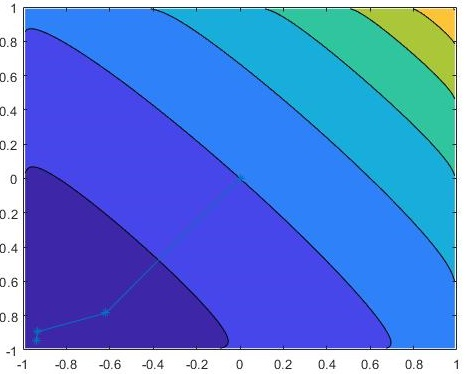
\includegraphics[width=0.24\textwidth]{code/100.jpg}}
   \subfloat {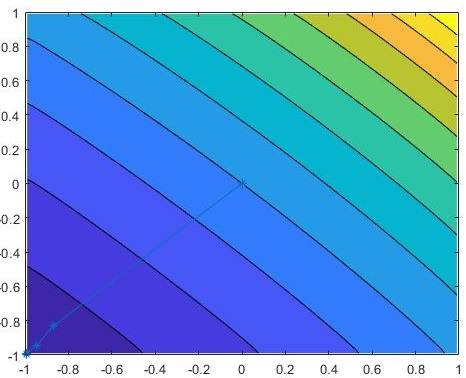
\includegraphics[width=0.24\textwidth]{code/1000.jpg}}
   \subfloat {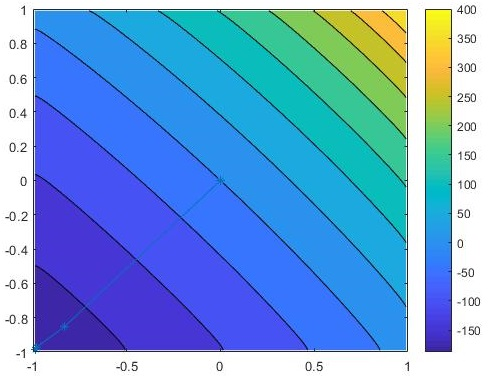
\includegraphics[width=0.24\textwidth]{code/500.jpg}}
   \caption{Contours of the objective function along with the trajectory of $x$ from Newton method with $\alpha = 0.01$, $\beta = 0.5$, $n=2$ and different $m$. From left to right, $m$ is set to 5, 100, 500 and 1000.}
   \label{fig:contours}
\end{figure}

After that we implemented the gradient method. Figure~\ref{fig:comp} shows a comparison between the gradient method and Newton's method in terms of the step size per iteration, $f(x^{k})-p^{*}$ per iteration and $f(x^{k})$ per iteration for $m=n=1000$, $\alpha = 0.01$ and $\beta = 0.5$. We took $p^{*}$ as the last computed value in the objective function for both methods. We notice that even though both methods are set to have the same precision or tolerance ($10^{-10}$) and maximum number of iterations, Newton's method was able to finish fast in 10 iterations while the gradient method took the maximum number of iterations (50). From the left column we can see clearly the quadratic convergence of Newton's method vs. the linear convergence of the gradient method. Experimenting with different problem sizes and different distributions from which we picked $A$ gave the same results and convergence rates. Increasing $\beta$ (up to 0.9) made the gradient method take longer to stabilize while it did not affect Newton's method. Increasing $\alpha$ (up to 0.9) has the same affect as increasing $\beta$ on both the gradient method and Newton's method in which case both methods took the 50 maximum iterations to exit.

\begin{figure}[!tbh]
\centering        
   \subfloat {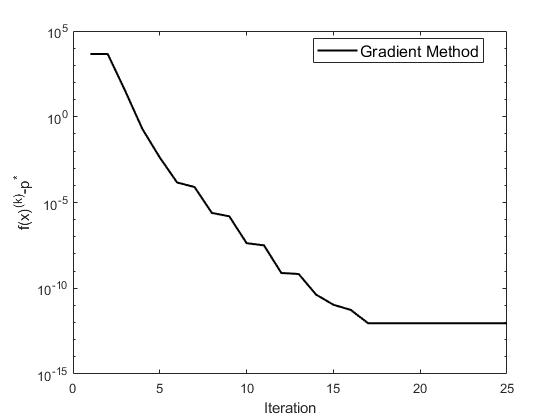
\includegraphics[width=0.33\textwidth]{code/p_grad.jpg}}
   \subfloat {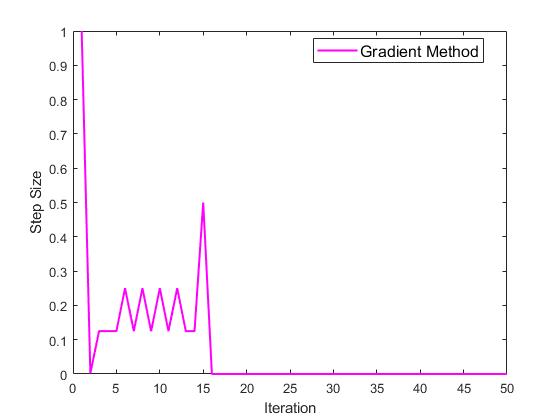
\includegraphics[width=0.33\textwidth]{code/step_grad.jpg}}
   \subfloat {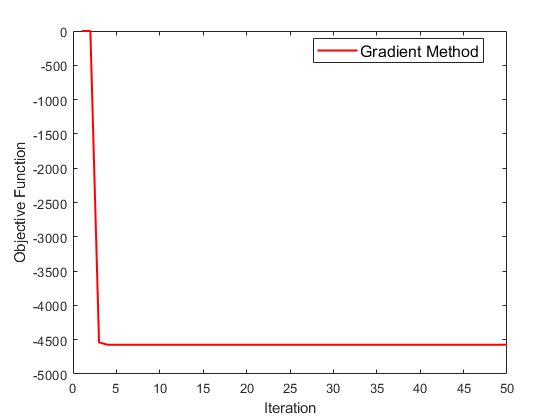
\includegraphics[width=0.33\textwidth]{code/obj_grad.jpg}}
   
   \subfloat {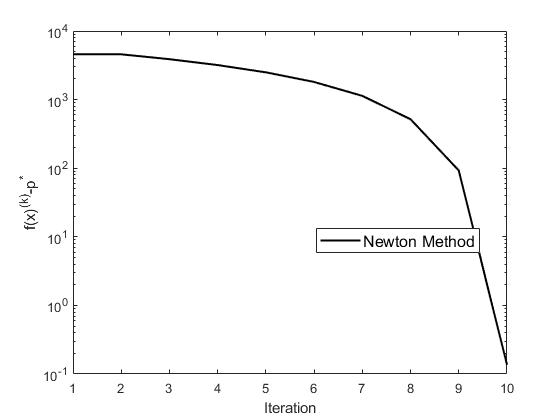
\includegraphics[width=0.33\textwidth]{code/p_new.jpg}}
   \subfloat {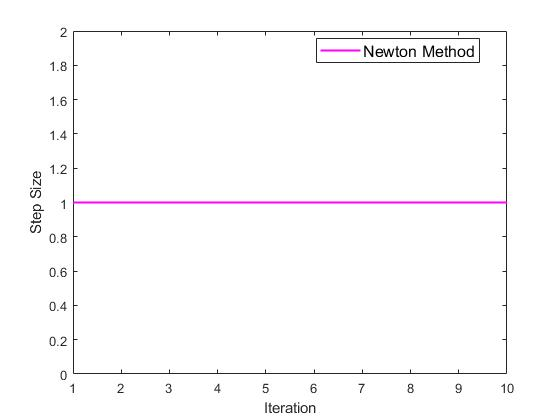
\includegraphics[width=0.33\textwidth]{code/step_new.jpg}}
   \subfloat {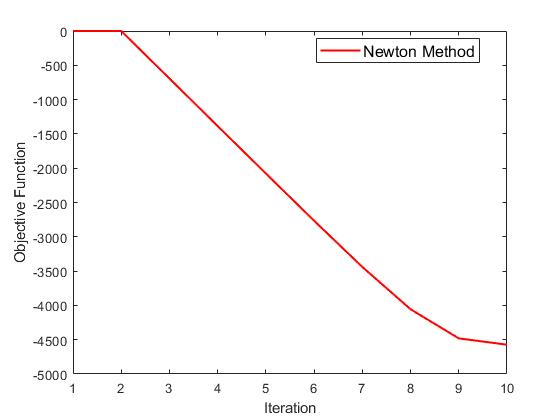
\includegraphics[width=0.33\textwidth]{code/obj_new.jpg}}
   
   \caption{Comparing gradient and Newton's methods in terms of step size per iteration, speed of convergence, and achieved objective function per iteration. Note the $x$-axis scale (i.e., number of iteration is different for both methods. Also,  $f(x^{k})-p^{*}$  is on a semi-log scale.}
   \label{fig:comp}
\end{figure}

\newpage
\paragraph{Gradient method code:}
The following listing shows the Gradient's method code used for generating the results 
\begin{lstlisting}
function [X,T,objFun] = Gradient_Method(Alpha, Beta, Func, Jac, isFeasible,  X0, MaxIt)   
    %apply Gradient metho and return the function, X for each iteration 
    %along with the step 
    %@Alpha backtracking line search alpha 
    %@Beta backtracking line search beta
    %@Func is the input function(s) for which we are seeking the roots    
    %@Jac is a function to evaluate the Jacobian
    %@Hesse is a function to evaluate the Hessain
    %@X0 is the initial guess     
    %@MaxIt is the max number of iterations     
    x = X0;    
    X = x';
    n = 1;
    tol = 1e-10;%tolerance
    T = 1;
    objFun = Func(X0);
    while n < MaxIt
        %1) compute function and gradient    
        myF = Func(x);
        objFun = [objFun, myF];
        myJ = Jac(x);
        
        %2) stopping criterion based gradient norm 
        if norm(myJ) < tol
            break;
        end
                
        t = 1;
        %do line search while respecting the constraints 
        %find the right t 
        while ~isFeasible(x-t*myJ)
             t = Beta*t;
        end        
        while Func(x-t*myJ) > myF - Alpha*t*(myJ'*myJ)
            t = Beta*t;
        end 
        
        
        %4) update 
        x = x - t*myJ;
        T = [T,t];
        X = [X; x'];
        n=n+1;
    end
    
    
end
\end{lstlisting}


\paragraph{Newton's method code:}
The following listing shows the Newton's method code used for generating the results 
\begin{lstlisting}
function [X,T,objFun] = Newton(Alpha, Beta, Func, Jac, Hesse , isFeasible,  X0, MaxIt)   
    %apply Newton method and return the function, X for each iteration  
    %along with the step 
    %@Alpha backtracking line search alpha 
    %@Beta backtracking line search beta
    %@Func is the input function(s) for which we are seeking the roots    
    %@Jac is a function to evaluate the Jacobian
    %@Hesse is a function to evaluate the Hessain
    %@X0 is the initial guess     
    %@MaxIt is the max number of iterations     
    x = X0;    
    X = x';
    n = 1;
    tol = 1e-10;%tolerance
    T = 1;
    objFun = Func(X0);
    while n < MaxIt        
        %1) compute newton step         
        myF = Func(x);
        objFun = [objFun, myF];
        myJ = Jac(x);        
        myH = Hesse(x);        
        sol = mldivide(-myH,myJ);

        %2) stopping criterion
        Lamda = myJ'*sol;
        if(Lamda*Lamda/2.0 < tol) %based on Newton decrement
        %if abs(normF(end)) < tol || abs(norm(X(end)) - norm(X(end-1))) <tol
            %based on the size of the norm and step size 
            break;
        end        
        
        %3) backtracking line search
        t = 1;
        %do line search while respecting the constraints 
        %find the right t 
        while ~isFeasible(x+t*sol)
             t = Beta*t;
        end        
        while Func(x+t*sol) > myF + Alpha*t*Lamda
            t = Beta*t;
        end 
        %4) update 
        x = x + t*sol;
        T = [T,t];
        X = [X; x'];
        n=n+1;
    end
end
\end{lstlisting}

\paragraph{Main code}
The following listing shows the main code that sets up the problems; contains the objective function, gradient and Hessain function calculations; call the gradient or Newton's methods; and plots the graphs. 

\begin{lstlisting}
clc;
clear;
close all;
disp('EEC 254 - HW6 - Problem 9.30:');
%%%%%%%%%%%%%%%%%%% Part a)
global A numRows numCols;
numRows = 1000;
numCols = 1000;
A = instance(numRows, numCols);%init matrix A
x = zeros(numCols,1);%init vector x
Alpha = 0.9;
Beta = 0.5;

[X_grad, steplen_grad, objFunc_grad] = Gradient_Method(Alpha,Beta, @Func, @Grad, @isFeasible, x, 50);
objFun_p_grad = objFunc_grad - objFunc_grad(end);

figure
semilogy(objFun_p_grad,'k', 'LineWidth',1.5);
xlabel('Iteration');
ylabel('f(x)^{(k)}-p^*');
label1 = 'Gradient Method';
lgd = legend(label1,'Location','best');
lgd.FontSize = 12;

figure
plot(steplen_grad,'m','LineWidth',1.5);
xlabel('Iteration');
ylabel('Step Size');
lgd = legend(label1,'Location','best');
lgd.FontSize = 12;

figure
plot(objFunc_grad,'r','LineWidth',1.5);
xlabel('Iteration');
ylabel('Objective Function');
lgd = legend(label1,'Location','best');
lgd.FontSize = 12;

if length(X_grad(1,:)) == 2
    %plot the contours of the domain if its 2d 
    %plotNorm(1,X_grad,@Func);
end

%%%%%%%%%%%%%%%%%%%%%%%%%%%%%%%%%%%%%%%%%%%%%%%%%%%%%%%%%%%%
[X_newton, steplen_newton, objFunc_newton] = Newton(Alpha,Beta, @Func, @Grad, @Hessain,@isFeasible, x, 50);
objFun_p_newton = objFunc_newton - objFunc_newton(end);

if length(X_newton(1,:)) == 2
    %plot the contours of the domain if its 2d 
    %plotNorm(2,X_newton,@Func);
end

figure
semilogy(objFun_p_newton,'k', 'LineWidth',1.5);
xlabel('Iteration');
ylabel('f(x)^{(k)}-p^*');
label1 = 'Newton Method';
lgd = legend(label1,'Location','best');
lgd.FontSize = 12;

figure
plot(steplen_newton,'m','LineWidth',1.5);
xlabel('Iteration');
ylabel('Step Size');
lgd = legend(label1,'Location','best');
lgd.FontSize = 12;

figure
plot(objFunc_newton,'r','LineWidth',1.5);
xlabel('Iteration');
ylabel('Objective Function');
lgd = legend(label1,'Location','best');
lgd.FontSize = 12;


disp('Done!!');


%%%%%%%%%%%%%%%%%%%%%%%%%%%%%%%%%%%%%%%%%%%%%%%%%%%%%%%%%%%
%%%%%%%%%%%%%%%%%%%%%%%%%%% Instance %%%%%%%%%%%%%%%%%%%%%%
%%%%%%%%%%%%%%%%%%%%%%%%%%%%%%%%%%%%%%%%%%%%%%%%%%%%%%%%%%%
function A = instance(numRows, numCols)
    %creating a problem instance 
    A = rand(numRows,numCols);    
    A=A./(2.0*max(max(A)));    
end

%%%%%%%%%%%%%%%%%%%%%%%%%%%%%%%%%%%%%%%%%%%%%%%%%%%%%%%%%%%
%%%%%%%%%%%%%%%%%%%%%%%%%Plot Contours %%%%%%%%%%%%%%%%%%%%
%%%%%%%%%%%%%%%%%%%%%%%%%%%%%%%%%%%%%%%%%%%%%%%%%%%%%%%%%%%
function plotNorm(fignum, X, func)
    v=[10.3,.01:1:900];
    xr=-0.99:0.005:0.99;
    n=length(xr);
    z=zeros(n,n);
    for i=1:n
        for j=1:n        
            z(i,j)=func([xr(i),xr(j)]);
        end
    end
    figure(fignum);
    contourf(xr,xr,z);
    ylim([-1 1]);
    xlim([-1 1]);
    hold 
    
    plot(X(:,1),X(:,2),'-*');
end

%%%%%%%%%%%%%%%%%%%%%%%%%%%%%%%%%%%%%%%%%%%%%%%%%%%%%%%%%%%
    %%%%%%%%%%%%%%%%%%%%%% Functions %%%%%%%%%%%%%%%%
%%%%%%%%%%%%%%%%%%%%%%%%%%%%%%%%%%%%%%%%%%%%%%%%%%%%%%%%%%%
function myVal = Func(x)
    global A numRows numCols
    %Evluate the function on x
    %x is a vector of length numCols 
    %A is numRows x numCols
    myVal = 0;
    for i=1:numRows
        myVal = myVal + log(1- dot(A(i,:),x));
    end
    for i=1:numCols
        myVal = myVal + log(1- x(i)*x(i));
    end    
    myVal = -myVal;
end
function myGrad = Grad(x)
    global A
    %Evluate the gradient on x    
    %using chain rule
    myGrad = A'*(1./(1-A*x)) - 1./(1+x) + 1./(1-x);
end
function myHessain = Hessain(x)
    global A    
    %Evluate the hessain on x    
    %using chain rule
    myHessain = A'*diag((1./(1-A*x)).^2)*A + diag(1./(1+x).^2 + 1./(1-x).^2); 
    
end
function fe = isFeasible(x)
    global A    
    %check if x is in the feasible region by checking the constraints 
    fe = true;
    if max(A*x) >= 1.0 %= to avoid numerical issues 
        fe = false;
    end
    
    if max(abs(x)) >= 1.0 
        fe = false;
    end

end
\end{lstlisting}
\bibliography{mybib}
\end{document}
